\documentclass{article}
\usepackage{fancyhdr}
\usepackage{geometry}
\usepackage{amsfonts}
\usepackage{amsthm}
\usepackage{tikz} % Add this line to include tikz package

% Set page margins
\geometry{margin=1in}

% Define fancy header
\pagestyle{fancy}
\fancyhf{}
\renewcommand{\headrulewidth}{0.4pt}
\fancyhead[L]{Patrick Brown}
\fancyhead[C]{Optimization - Homework 1}
\fancyhead[R]{\thepage}

% Define a new environment for answers
\newenvironment{answer}
    {\par\noindent\textbf{Answer:}\par}
    {\par}

\begin{document}

\begin{center}
\Large\textbf{The University of Texas at Austin}\\[0.5em]
\large\textbf{Optimization}\\[0.5em]
\large\textbf{Homework 1}
\end{center}

\vspace{1em}

\textbf{Instructors:} Constantine Caramanis, Sujay Sanghavi

\vspace{1em}

\textbf{Submitting solutions:} Please submit your solutions as a single pdf file. If you have code or figures, please include these in the pdf.

\section{Convex Sets, Convex Functions, Preservation of Convexity}

\begin{enumerate}
    \item 
    \begin{enumerate}
        \item 
        \begin{answer}
        To show that the intersection of convex sets is convex, we will prove that the intersection of any finite number of convex sets is convex. Let $\{C_i\}_{i=1}^n$ be a collection of convex sets, and let $C = \bigcap_{i=1}^n C_i$ be their intersection.

        1) First, we need to show that $C$ is non-empty. This is assumed implicitly, as the intersection of convex sets can be empty (e.g., two disjoint convex sets).

        2) Let $\mathbf{x}, \mathbf{y} \in C$. This means $\mathbf{x}, \mathbf{y} \in C_i$ for all $i = 1, 2, ..., n$.

        3) To prove $C$ is convex, we need to show that for any $\lambda \in [0,1]$, the point $\mathbf{z} = \lambda\mathbf{x} + (1-\lambda)\mathbf{y}$ is also in $C$.

        4) For each $C_i$:
           - Since $C_i$ is convex and $\mathbf{x}, \mathbf{y} \in C_i$, we know that $\mathbf{z} = \lambda\mathbf{x} + (1-\lambda)\mathbf{y} \in C_i$ for any $\lambda \in [0,1]$.

        5) Since $\mathbf{z} \in C_i$ for all $i = 1, 2, ..., n$, we can conclude that $\mathbf{z} \in \bigcap_{i=1}^n C_i = C$.

        6) Therefore, for any two points in $C$ and any $\lambda \in [0,1]$, the convex combination of these points is also in $C$.

        This satisfies the definition of a convex set, proving that $C$ is convex. Thus, the intersection of any finite number of convex sets is convex.

        Note: This proof can be extended to the intersection of an infinite number of convex sets by considering arbitrary subsets of the intersection and applying the same logic.
        \end{answer}

        \item 
        \begin{answer}
        An example where the union of two convex sets is not convex:
        
        Consider two disjoint circles in $\mathbb{R}^2$. Each circle is a convex set, but their union is not convex because a line segment connecting a point in one circle to a point in the other circle would not be entirely contained within the union.
        
        \begin{center}
        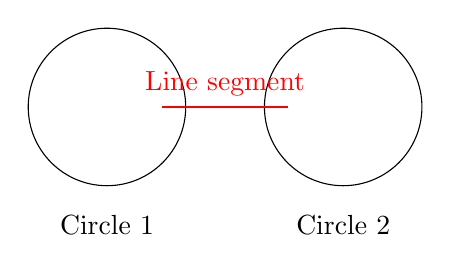
\begin{tikzpicture}
            % Draw two circles
            \draw (0,0) circle (1cm);
            \draw (3,0) circle (1cm);
            
            % Draw a line segment between the circles
            \draw[red, thick] (0.7,0) -- (2.3,0);
            
            % Add labels
            \node at (0,-1.5) {Circle 1};
            \node at (3,-1.5) {Circle 2};
            \node[red] at (1.5,0.3) {Line segment};
        \end{tikzpicture}
        \end{center}
        
        As shown in the figure, the red line segment connecting points in the two circles is not entirely contained within the union of the circles, demonstrating that the union is not convex.
        \end{answer}

        \item 
        \begin{answer}
        To show that the maximum of convex functions is convex, let $f_1$ and $f_2$ be convex functions, and $f_{\max}(x) = \max\{f_1(x), f_2(x)\}$.
        
        For any $\mathbf{x}, \mathbf{y}$ and $\lambda \in [0,1]$:
        
        $f_{\max}(\lambda\mathbf{x} + (1-\lambda)\mathbf{y})$
        $= \max\{f_1(\lambda\mathbf{x} + (1-\lambda)\mathbf{y}), f_2(\lambda\mathbf{x} + (1-\lambda)\mathbf{y})\}$
        
        $\leq \max\{\lambda f_1(\mathbf{x}) + (1-\lambda)f_1(\mathbf{y}), \lambda f_2(\mathbf{x}) + (1-\lambda)f_2(\mathbf{y})\}$
        
        $\leq \lambda \max\{f_1(\mathbf{x}), f_2(\mathbf{x})\} + (1-\lambda) \max\{f_1(\mathbf{y}), f_2(\mathbf{y})\}$
        
        $= \lambda f_{\max}(\mathbf{x}) + (1-\lambda) f_{\max}(\mathbf{y})$
        
        This proves that $f_{\max}$ satisfies the definition of convexity, and thus the maximum of convex functions is convex.
        \end{answer}
    \end{enumerate}

    \section{More Convex Sets, Convex Functions, Preservation of Convexity}

    \begin{enumerate}
        \item 
        \begin{answer}
        An example where the minimum of two convex functions is not convex:
        
        Consider $f_1(x) = x^2$ and $f_2(x) = (x-2)^2$. Both are convex functions.
        Let $f_{\min}(x) = \min\{f_1(x), f_2(x)\}$.
        
        The sub-level set of $f_{\min}$ for some $c > 0$ is:
        $S_c = \{x : f_{\min}(x) \leq c\} = \{x : \min\{x^2, (x-2)^2\} \leq c\}$
        
        $f_{\min}(x)$ is not convex because it forms a "V" shape with a non-convex kink at $x=1$, where the two parabolas intersect.

        \begin{center}
            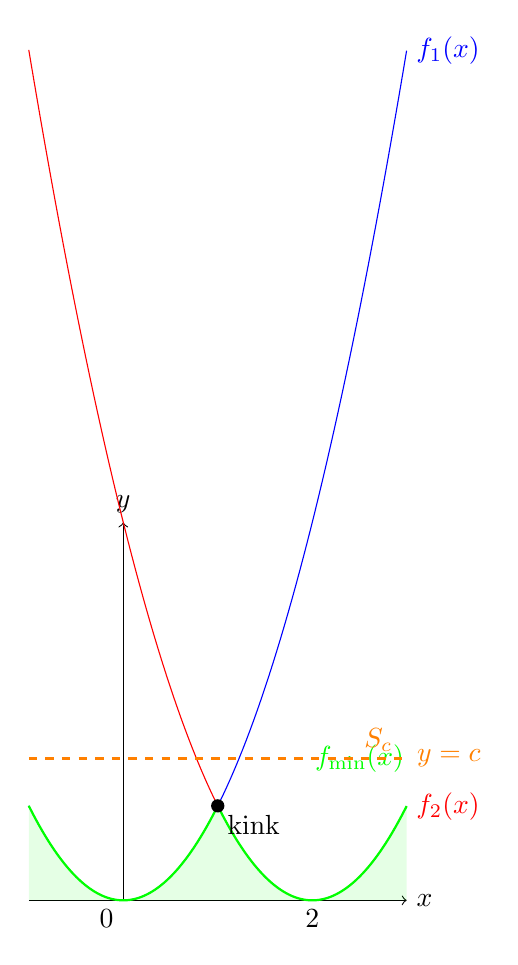
\begin{tikzpicture}[scale=1.2]
                % Draw axes
                \draw[->] (-1,0) -- (3,0) node[right] {$x$};
                \draw[->] (0,0) -- (0,4) node[above] {$y$};
                
                % Draw f1(x) = x^2
                \draw[blue, domain=-1:3, samples=100] plot (\x, {\x*\x}) node[right] {$f_1(x)$};
                
                % Draw f2(x) = (x-2)^2
                \draw[red, domain=-1:3, samples=100] plot (\x, {(\x-2)*(\x-2)}) node[right] {$f_2(x)$};
                
                % Draw f_min(x)
                \draw[green, thick, domain=-1:1, samples=100] plot (\x, {\x*\x});
                \draw[green, thick, domain=1:3, samples=100] plot (\x, {(\x-2)*(\x-2)});
                
                % Shade the area below f_min(x)
                \fill[green, opacity=0.1] (-1,0) -- plot[domain=-1:1] (\x, {\x*\x}) -- 
                    plot[domain=1:3] (\x, {(\x-2)*(\x-2)}) -- (3,0) -- cycle;
                
                % Label f_min(x)
                \node[green] at (2.5,1.5) {$f_{\min}(x)$};
                
                % Mark the non-convex kink
                \fill[black] (1,1) circle (2pt);
                \node[below right] at (1,1) {kink};
                
                % Label axes
                \node[below left] at (0,0) {$0$};
                \node[below] at (2,0) {$2$};
                
                % Draw a sample sub-level set
                \draw[orange, thick, dashed] (-1,1.5) -- (3,1.5) node[right] {$y=c$};
                \node[orange] at (2.7,1.7) {$S_c$};
            \end{tikzpicture}
        \end{center}
        
        The shaded area represents the region where $f_{\min}(x) \leq y$ for any $y$. The dashed orange line shows a sample sub-level set $S_c$ for some $c > 0$. Note that this sub-level set is not convex, as it consists of two disjoint intervals when $c < 1$.
        
        This example demonstrates that the minimum of two convex functions is not necessarily convex, as evidenced by the non-convex kink in $f_{\min}(x)$ and the potentially non-convex sub-level sets.
        \end{answer}
        
        
        \begin{answer}
        An example of two closed convex sets that are disjoint but cannot be strictly separated:

        Consider the following two sets in $\mathbb{R}^2$:

        $A = \{(x, y) : y \geq e^x\}$
        $B = \{(x, y) : y \leq 0\}$

        Both $A$ and $B$ are closed convex sets:
        - $A$ is the epigraph of the exponential function, which is convex.
        - $B$ is a half-space, which is convex.

        These sets are disjoint because $e^x > 0$ for all $x \in \mathbb{R}$, so no point can simultaneously satisfy $y \geq e^x$ and $y \leq 0$.

        However, they cannot be strictly separated because for any $\epsilon > 0$, we can find points in $A$ and $B$ that are less than $\epsilon$ apart:

        For any $x < 0$ with large magnitude:
        - The point $(x, e^x)$ is in $A$
        - The point $(x, 0)$ is in $B$
        - The distance between these points is $e^x$, which approaches 0 as $x \to -\infty$

        \begin{center}
        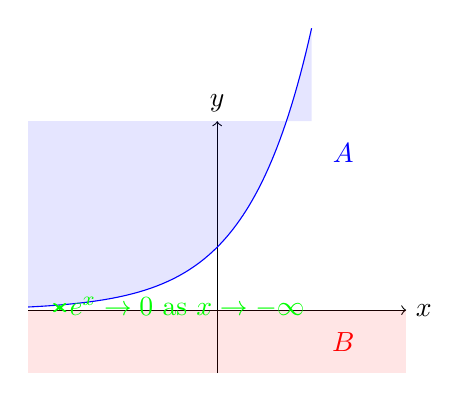
\begin{tikzpicture}[scale=0.8]
            % Draw axes
            \draw[->] (-3,0) -- (3,0) node[right] {$x$};
            \draw[->] (0,-1) -- (0,3) node[above] {$y$};
            
            % Draw set A (exponential function)
            \draw[blue, domain=-3:1.5, samples=100] plot (\x, {exp(\x)});
            \fill[blue, opacity=0.1] (-3,3) -- plot[domain=-3:1.5] (\x, {exp(\x)}) -- (1.5,3) -- cycle;
            
            % Draw set B (y <= 0)
            \fill[red, opacity=0.1] (-3,-1) rectangle (3,0);
            
            % Labels
            \node[blue] at (2,2.5) {$A$};
            \node[red] at (2,-0.5) {$B$};
            
            % Point out the closeness
            \draw[<->, green, thick] (-2.5,0) -- (-2.5,0.08);
            \node[green, right] at (-2.5,0.04) {$e^x \to 0$ as $x \to -\infty$};
        \end{tikzpicture}
        \end{center}

        This example demonstrates that while $A$ and $B$ are disjoint closed convex sets, they cannot be strictly separated because they get arbitrarily close to each other as $x \to -\infty$.
        \end{answer}
        \item 
        \begin{answer}
        To prove that any sub-level set of a convex function is convex:
    
        Let $f: \mathbb{R}^n \to \mathbb{R}$ be a convex function, and $L_c = \{x : f(x) \leq c\}$ be a sub-level set for some $c \in \mathbb{R}$.
    
        1) Take any two points $x_1, x_2 \in L_c$. This means $f(x_1) \leq c$ and $f(x_2) \leq c$.
        2) Consider any point $z = \lambda x_1 + (1-\lambda)x_2$, where $\lambda \in [0,1]$.
        3) By the definition of convexity: $f(z) \leq \lambda f(x_1) + (1-\lambda)f(x_2)$
        4) Since $f(x_1) \leq c$ and $f(x_2) \leq c$, we have:
           $f(z) \leq \lambda c + (1-\lambda)c = c$
        5) Therefore, $z \in L_c$
    
        This proves that any sub-level set of a convex function is convex.
    
        Example showing the converse is NOT true:
    
        Consider the function $f(x) = -x^2$. This function is concave (not convex).
    
        Its sub-level sets are of the form:
        $L_c = \{x : -x^2 \leq c\}$ or $\{x : x^2 \geq -c\}$
    
        For $c < 0$, these sets are intervals of the form $[-\sqrt{-c}, \sqrt{-c}]$, which are convex.
        For $c \geq 0$, the set is all of $\mathbb{R}$, which is also convex.
    
        Thus, all sub-level sets of this non-convex function are convex.
    
        \begin{center}
        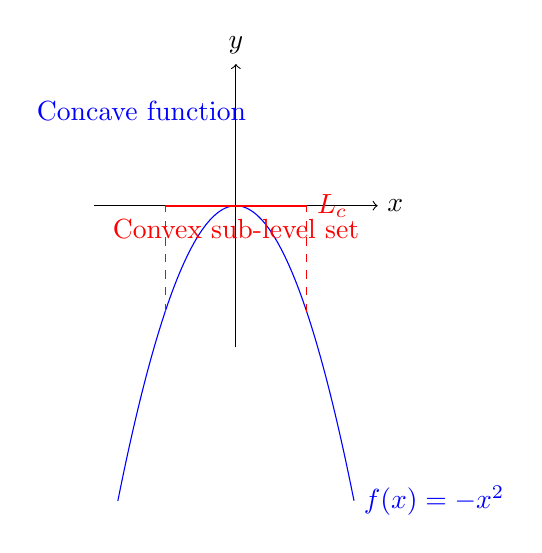
\begin{tikzpicture}[scale=0.6]
            % Draw axes
            \draw[->] (-3,0) -- (3,0) node[right] {$x$};
            \draw[->] (0,-3) -- (0,3) node[above] {$y$};
            
            % Draw f(x) = -x^2
            \draw[blue, domain=-2.5:2.5, samples=100] plot (\x, {-\x*\x}) node[right] {$f(x) = -x^2$};
            
            % Draw a sample sub-level set
            \draw[red, thick] (-1.5,0) -- (1.5,0) node[right] {$L_c$};
            \draw[red, dashed] (-1.5,-2.25) -- (-1.5,0);
            \draw[red, dashed] (1.5,-2.25) -- (1.5,0);
            
            % Labels
            \node[blue] at (-2,2) {Concave function};
            \node[red] at (0,-0.5) {Convex sub-level set};
        \end{tikzpicture}
        \end{center}
    
        This example demonstrates that having convex sub-level sets does not guarantee that the function itself is convex.
        \end{answer}
    \end{enumerate}
\end{enumerate}

\section{Half-Space Representation of Points Closer to v1 than v2}

\begin{enumerate}
    \item Consider two points, $v_1, v_2 \in \mathbb{R}^n$. In this exercise you will show that there exists a vector $c \in \mathbb{R}^n$ and a scalar $d \in \mathbb{R}$ such that
    
    $\{x : ||x - v_1||_2 \leq ||x - v_2||_2\} = \{x : c^T x \leq d\}$.

    \begin{answer}
    Let's address each part of the question:

    \begin{enumerate}
        \item Two dimensions: consider the above problem in two dimensions, where $v_1 = (-1,0)^T$, and $v_2 = (1,0)^T$. Draw the set of points that are closer to $v_1$ than $v_2$, by shading the plane. This should be a half-space!

        Here's a visualization of this 2D example:
        
        \begin{center}
            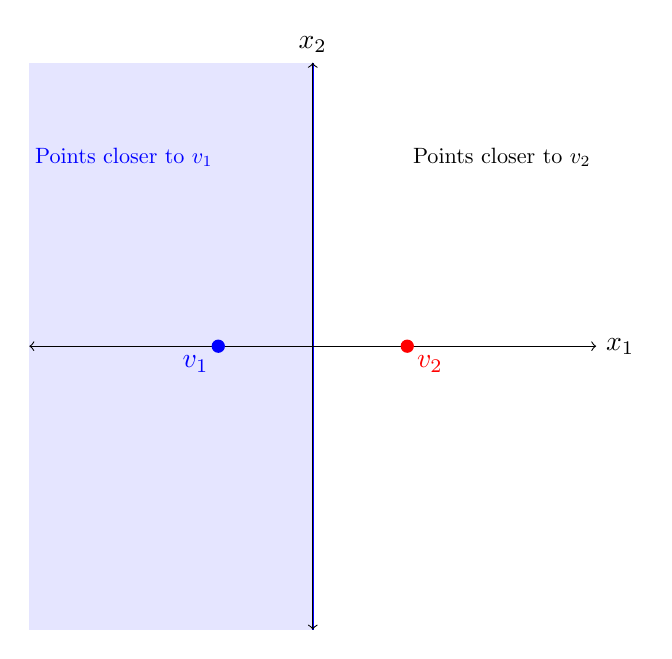
\begin{tikzpicture}[scale=1.2]
                % Shade the left half-plane
                \fill[blue!10] (-3,-3) rectangle (0,3);
                
                % Draw the dividing line
                \draw[blue, thick] (0,-3) -- (0,3);
                
                % Draw axes on top of the shaded area
                \draw[<->] (-3,0) -- (3,0) node[right] {$x_1$};
                \draw[<->] (0,-3) -- (0,3) node[above] {$x_2$};
                
                % Plot points v1 and v2
                \fill[blue] (-1,0) circle (2pt) node[below left] {$v_1$};
                \fill[red] (1,0) circle (2pt) node[below right] {$v_2$};
                
                % Add labels
                \node[blue, scale=0.8] at (-2,2) {Points closer to $v_1$};
                \node[scale=0.8] at (2,2) {Points closer to $v_2$};
            \end{tikzpicture}
            \end{center}

        In this visualization:
        - The blue shaded area represents the half-space containing all points closer to $v_1$ than to $v_2$.
        - The red line is the perpendicular bisector of the line segment joining $v_1$ and $v_2$, representing the boundary where points are equidistant from $v_1$ and $v_2$.
        - $v_1 = (-1, 0)$ is shown in blue, and $v_2 = (1, 0)$ is shown in red.

        \item For the above example, find the two-dimensional vector $c = (c_1, c_2)^T$ and the scalar $d$ that describes the shaded region from the above. So in other words, the shaded region you drew must correspond to:
        
        $\{(x_1, x_2)^T : c_1x_1 + c_2x_2 \leq d\}$.

        For this example where $v_1 = (-1, 0)^T$ and $v_2 = (1, 0)^T$:
        
        $c = 2(v_2 - v_1) = 2((1, 0)^T - (-1, 0)^T) = (4, 0)^T$
        So, $c_1 = 4$ and $c_2 = 0$

        $d = v_2^Tv_2 - v_1^Tv_1 = 1^2 + 0^2 - (-1)^2 - 0^2 = 0$
        
        Therefore, the half-space is described by:
        $\{(x_1, x_2)^T : 4x_1 + 0x_2 \leq 0\}$ or simply $\{(x_1, x_2)^T : x_1 \leq 0\}$
        
        This corresponds to the left half-plane in our visualization.

        \item Finally, generalize the above. For general points $v_1, v_2 \in \mathbb{R}^n$, find a vector $c \in \mathbb{R}^n$ and a scalar $d \in \mathbb{R}$ such that
        
        $\{x : ||x - v_1||_2 \leq ||x - v_2||_2\} = \{x : c^T x \leq d\}$.

        To prove this for general $v_1, v_2 \in \mathbb{R}^n$, we'll follow these steps:

        1) Start with the inequality: $||x - v_1||_2 \leq ||x - v_2||_2$

        2) Square both sides (since both sides are non-negative, this preserves the inequality):
        $(x - v_1)^T(x - v_1) \leq (x - v_2)^T(x - v_2)$

        3) Expand:
        $x^Tx - 2v_1^Tx + v_1^Tv_1 \leq x^Tx - 2v_2^Tx + v_2^Tv_2$

        4) The $x^Tx$ terms cancel out:
        $-2v_1^Tx + v_1^Tv_1 \leq -2v_2^Tx + v_2^Tv_2$

        5) Rearrange:
        $2(v_2 - v_1)^Tx \leq v_2^Tv_2 - v_1^Tv_1$

        6) Now we can identify:
        $c = 2(v_2 - v_1)$
        $d = v_2^Tv_2 - v_1^Tv_1$

        7) Let's plug these back into the inequality $c^T x \leq d$ to verify:
        $[2(v_2 - v_1)]^T x \leq v_2^Tv_2 - v_1^Tv_1$
        $2(v_2 - v_1)^T x \leq v_2^Tv_2 - v_1^Tv_1$

        This is exactly the inequality we derived in step 5, confirming that our expressions for c and d are correct.

        Thus, we have shown that:
        $\{x : ||x - v_1||_2 \leq ||x - v_2||_2\} = \{x : c^T x \leq d\}$

where $c = 2(v_2 - v_1)$ and $d = v_2^Tv_2 - v_1^Tv_1$.

        This proves that the set of points in $\mathbb{R}^n$ that are closer to point $v_1$ than to point $v_2$ form a half-space for any dimension $n$.
    \end{enumerate}
    \end{answer}
\end{enumerate}

\end{document}